\documentclass{ctpro}

\title{ACM算法与微应用实验室2021年11月月赛题目}
\date{2021年12月1日}

\begin{document}
\maketitle
\addproblem{pro1}{1000}{128}{传统}{AgOH}
\addproblem{pro2}{1000}{128}{传统}{AgOH}
\addproblem{三斜求积术}{1000}{128}{传统}{AgOH}
\addproblem{子树大小}{1000}{128}{传统}{AgOH}
\addproblem{pro5}{1000}{128}{传统}{AgOH}
\addproblem{pro6}{1000}{128}{传统}{AgOH}

\section*{比赛信息}
\ctinfotab{ACM\ |个人赛|不封榜}{C/C++,Python,Java}{3}

\section*{题目概况}
\problemtab

\section*{编译命令}
参见OJ帮助

\section*{注意事项}
\begin{itemize}
	\item C/C++中函数main()的返回值类型必须是int,程序正常结束时的返回值必须是0。
	\item C/C++代码必须完全符合GNU C/C++ 标准,不能使用诸如绘图、Win32API、中断调用、硬件操作或与操作系统相关的API。
	\item C/C++代码中允许使用STL类库。
\end{itemize}

\paragraph*{} 祝大家取得好成绩!

\makeproblem
\section*{题目描述}
\section*{输入格式}
\section*{输出格式}
\section*{输入输出样例}

\makeproblem
\section*{题目描述}
\section*{输入格式}
\section*{输出格式}
\section*{输入输出样例}

\makeproblem
\section*{题目描述}
给出一个三角形三条边的边长,请算出这个三角形的面积。

\section*{输入格式}
第一行,一个整数 $t~(1 \leq t \leq 10^5)$,代表共有 $t$ 组数据。

对于每组数据:

\indent \indent 一行,三个整数 $a,b,c~(1 \leq a,b,c \leq 10^4)$,代表三角形三条边的长度。

\section*{输出格式}
对于每组数据,在一行内输出一个实数(四舍五入保留 $2$ 位小数),代表答案。


\section*{输入输出样例}
\testcasetab
{
	3 \par
	3 3 3\par
	3 4 5\par
	2 3 3
}
{
	3.90\par
	6.00\par
	2.83\par
}

\section*{说明/提示}
\textbf{海伦公式}
\begin{quotation}
	海伦公式又译作希伦公式、海龙公式、希罗公式、海伦-秦九韶公式。它是利用三角形的三条边的边长直接求三角形面积的公式。

	假设在平面内,有一个三角形,边长分别为 $a,b,c$,三角形的面积 $S$ 可由以下公式求得:

	$$S=\sqrt{p(p-a)(p-b)(p-c)}$$

	其中 $p$ 为三角形的半周长(周长的一半):

	$$p=\cfrac{a+b+c}{2}$$
\end{quotation}

\makeproblem
\section*{题目描述}
对于一棵树,有定义如下:

\begin{definition}[树的大小]
	树中存在的结点的数量叫做这棵树的大小。
\end{definition}

给定一棵树,请分别计算出以各结点作为根结点时各子树的大小。

\section*{输入格式}
第一行,两个整数 $n~(1 \leq n \leq 10^4)$,代表给定的树的大小。

接下来的 $n-1$ 行,每行两个整数 $u,v~(1 \leq u,v \leq n)$,代表结点 $u$ 与结点 $v$ 之间有一条边。

\section*{输出格式}
输出共 $n$ 行,每行 $n$ 个整数 $s_1,s_2,\cdots,s_n$。$s_i$ 代表以 $i$ 为根结点的子树的大小。

\section*{输入输出样例}
\testcasetab
{
	5\par
	1 2\par
	1 3\par
	2 4\par
	2 5
}
{
	5 3 1 1 1\par
	2 5 1 1 1\par
	4 3 5 1 1\par
	2 4 1 5 1\par
	2 4 1 1 5
}

\section*{说明/提示}
分别以 $1 \sim 5$ 号结点作为根结点时,各子树大小:
\begin{figure}
	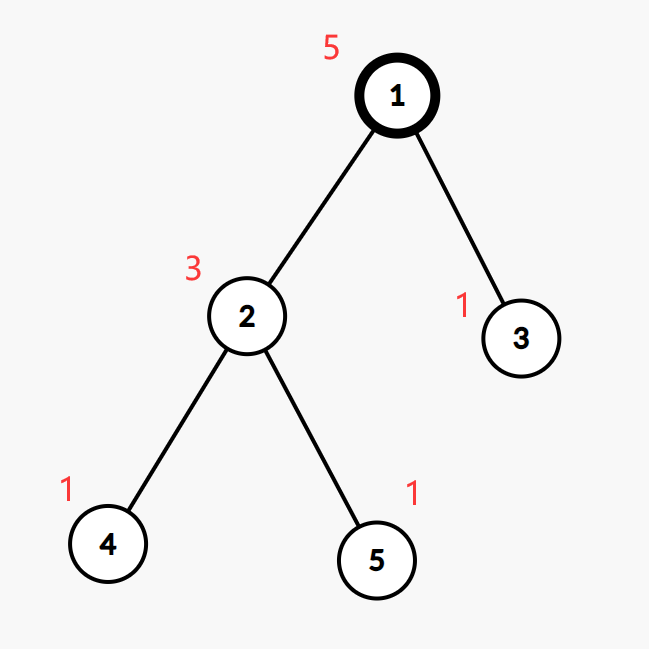
\includegraphics[scale=0.14]{images/D_1.png}
	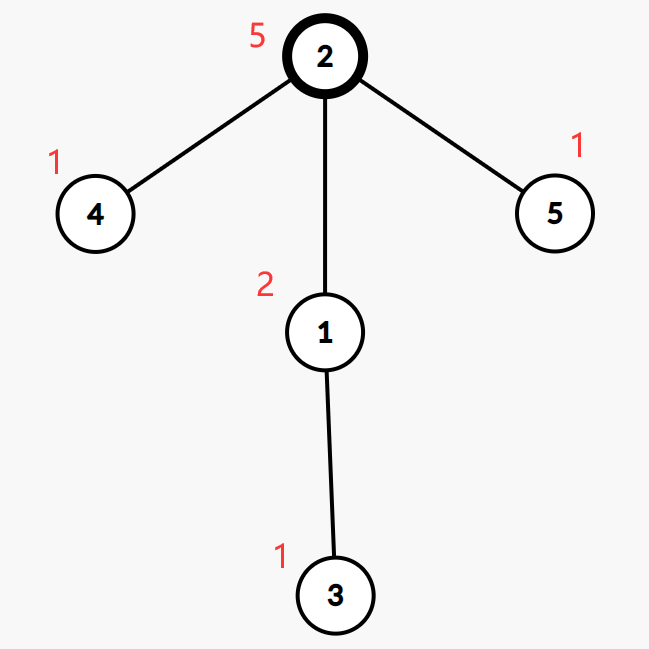
\includegraphics[scale=0.14]{images/D_2.png}
	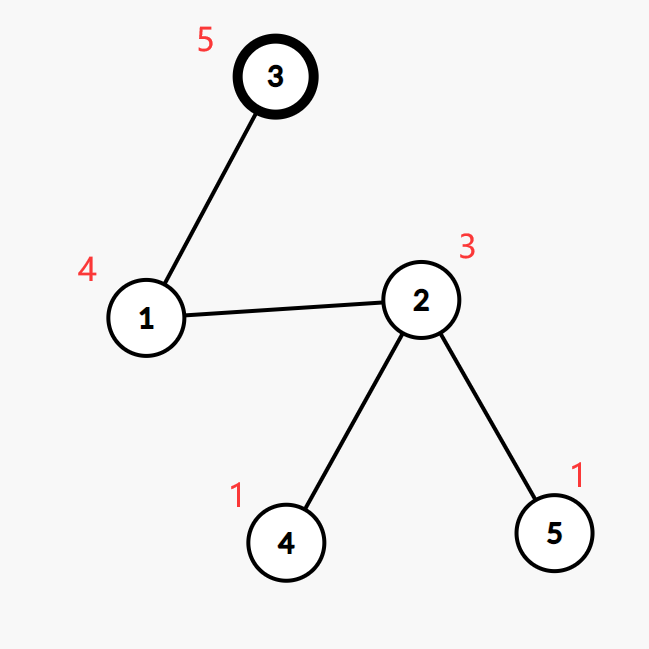
\includegraphics[scale=0.14]{images/D_3.png}
	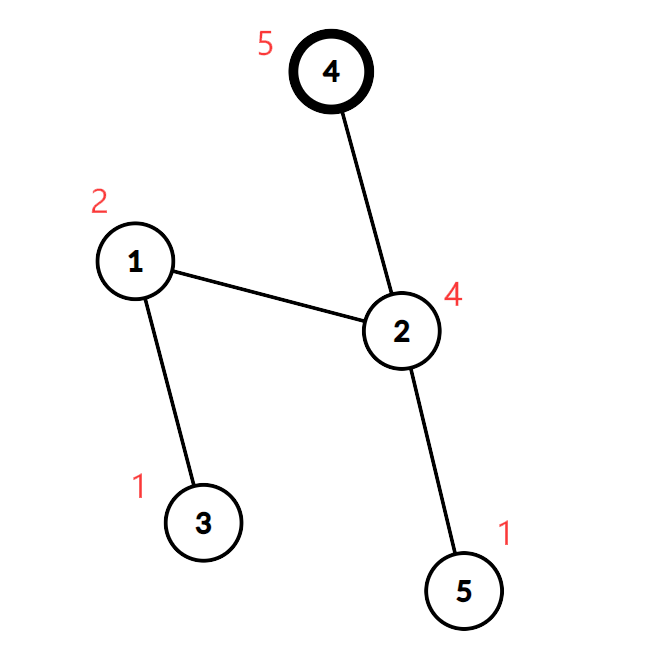
\includegraphics[scale=0.14]{images/D_4.png}
	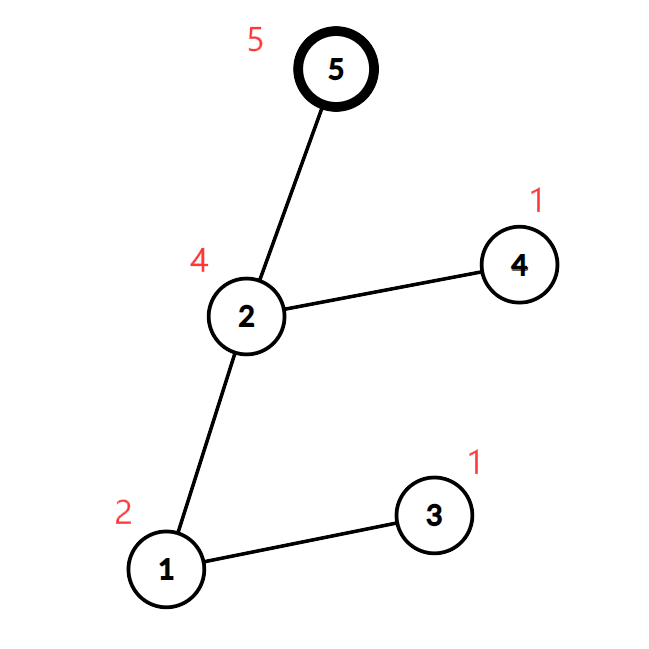
\includegraphics[scale=0.14]{images/D_5.png}
\end{figure}

\makeproblem
\section*{题目描述}
\section*{输入格式}
\section*{输出格式}
\section*{输入输出样例}

\makeproblem
\section*{题目描述}
\section*{输入格式}
\section*{输出格式}
\section*{输入输出样例}

\end{document}